\subsection{Forward stepwise selection}

The first method applied is the forward stepwise selection. In particular, the algorithm variant employed uses the \textit{p-value} as entrance criterion and the \textit{akaike information criterion} (AIC) as comparison metric between models. The model obtained is shown in \Tab~\ref{table:ForwardModelSummary}.

\begin{table}[H]
	\centering
	\begin{tabular}{|| l | r | r ||} 
		\hline
		\multicolumn{3}{|c|}{Equation} \\
		\hline
		Variable's coefficient & Estimated value & p value \\
		\hline
		intercept & -3.63 & 2e-16 \\
		MIN & 0.24 & 2e-16 \\
		FTM & 1.72 & 2e-16 \\
		3P MADE & 0.27 & 0.5716 \\
		FG\% & 0.06 & 2e-16 \\
		TOV & 1.57 & 2e-16 \\
		AST & -0.36 & 1.32e-13 \\
		DREB & -0.26 & 1.34e-05 \\
		3P\% & 0.01 & 4.07e-05 \\
		OREB & 0.29 & 0.0023 \\
		STL & -0.39 & 0.0059 \\
		3PA & 0.36 & 0.0490 \\
		BLK & -0.18 & 0.0919 \\
		GP & -0.39e-2 & 0.0935 \\
		\hline
	\end{tabular}
	\caption{Forward stepwise selection output model.}
	\label{table:ForwardModelSummary}
\end{table}

As expected, ``MIN'' and ``FTM'' are included, which resulted to be important from the preliminary analysis as well. However, there are three variables that are not significantly different from 0, with a p-value threshold of $5\%$.

\textbf{Bootstrap Statistical Inference}

On the obtained model we used the Bootstrap technique in order to perform statistical inference on the model coefficients. In \Tab~\ref{table:ForwardModelSummary} it is possible to see the results, that are coherent with the previous ones. This also shows that the gaussian approximation for the error is valid in this case. \todo{mettiamo R=1000?}

\begin{table}[H]
	\centering
	\begin{tabular}{|| l | r | r ||} 
		\hline
		\multicolumn{3}{|c|}{Equation} \\
		\hline
		Variable's coefficient & Estimated value & p value \\
		\hline
		intercept & -3.63 & 1e-3 \\
		MIN & 0.24 & 0.00 \\
		FTM & 1.72 & 0.00 \\
		3P MADE & 0.27 & 0.584 \\
		FG\% & 0.06 & 0.01e-1 \\
		TOV & 1.57 & 0.000 \\
		AST & -0.36 & 0.001 \\
		DREB & -0.26 & 0.001 \\
		3P\% & 0.01 & 0.000 \\
		OREB & 0.29 & 0.007 \\
		STL & -0.39 & 0.011 \\
		3PA & 0.36 & 0.055 \\
		BLK & -0.18 & 0.092 \\
		GP & -0.39e-2 & 0.093 \\
		\hline
	\end{tabular}
	\caption{Boostrap results on forward stepwise selection output model.}
	\label{table:BootForwardModel}
\end{table}

\vspace{0.2cm}
\noindent
\textbf{Final Forward Model}

The final forward model, shown in \Tab~\ref{table:ForwardFinalModelSummary}, is obtained removing the non significant variables. Instead, in \Fig~\ref{fig:ForwardFinalModelResiduals} and \Fig~\ref{fig:ForwardFinalModelResidualsDist} it is possible to see the plots of the residuals, that have a gaussian shape with 0 mean. This means that the model is likely adequate for our purposes.

\begin{table}[H]
	\centering
	\begin{tabular}{|| l | r | r ||} 
		\hline
		\multicolumn{3}{|c|}{Equation} \\
		\hline
		Variable's coefficient & Estimated value & p value \\
		\hline
		intercept & -3.74 & 2e-16 \\
		MIN & 0.24 & 2e-16 \\
		FTM & 1.72 & 2e-16 \\
		TOV & 1.55 & 2e-16 \\
		AST & -0.35 & 4.58e-13 \\
		FG\% & 0.06 & 2e-16 \\
		DREB & -0.29 & 1.38e-17 \\
		3P\% & 0.01 & 1.64e-05 \\
		OREB & 0.29 & 0.0024 \\
		STL & -0.40 & 0.0051 \\
		3PA & 0.47 & 2e-16 \\
		\hline
	\end{tabular}
	\caption{Final sorward stepwise selection model summary.}
	\label{table:ForwardFinalModelSummary}
\end{table}

\begin{figure}[H]
	\centering
	\begin{subfigure}{.6\textwidth}
		\centering
		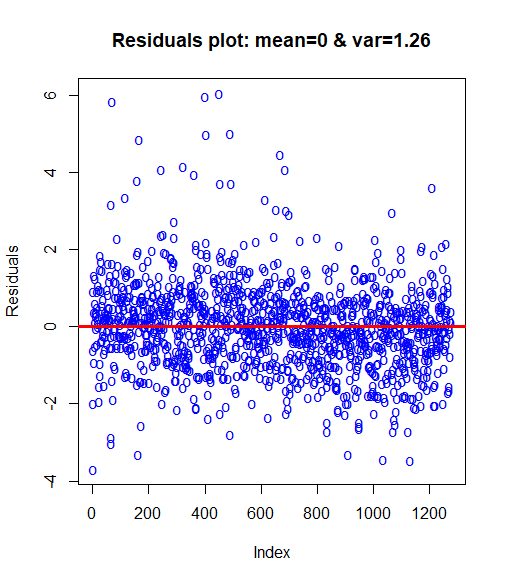
\includegraphics[width=0.6\linewidth]{ImageFiles/Regression/Forward/ForwardFinalModelResiduals}
		\caption{}
		\label{fig:ForwardFinalModelResiduals}
	\end{subfigure}%
	\begin{subfigure}{.6\textwidth}
		\centering
		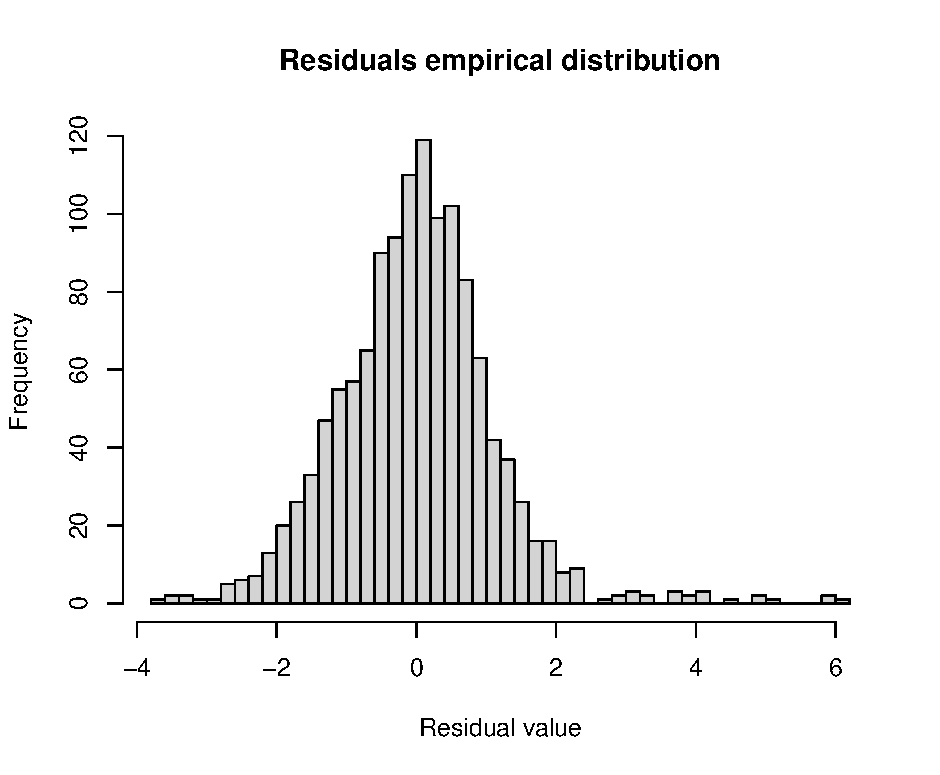
\includegraphics[width=0.6\linewidth]{ImageFiles/Regression/Forward/ForwardFinalModelResidualsDist}
		\caption{}
		\label{fig:ForwardFinalModelResidualsDist}
	\end{subfigure}
	\caption{Final Forward stepwise selection model. (a)Forward stepwise selection model residuals. (b)Forward stepwise selection residuals histogram.}
	\label{fig:FinalFSSM}
\end{figure}

